
\subsection{thesis proposal}

\begin{figure}
	\centering
	\begin{subfigure}[b]{0.7\textwidth}
		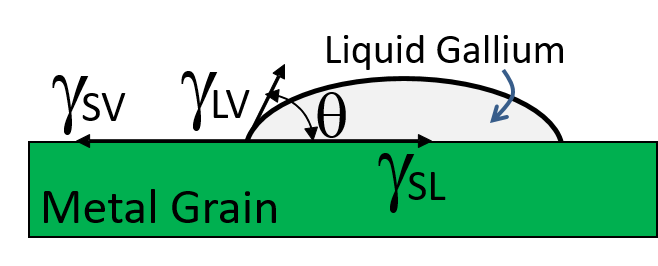
\includegraphics[width=\textwidth,trim={0 0 0 2cm}]{youngs-ga}
	%	\caption{Interfacial tensions on Ga drop on solid surface}
		\label{fig:youngs-ga}
	\end{subfigure}
	%add desired spacing between images, e. g. ~, \quad, \qquad, \hfill etc. 
	%(or a blank line to force the subfigure onto a new line)
	\begin{subfigure}[b]{0.7\textwidth}
		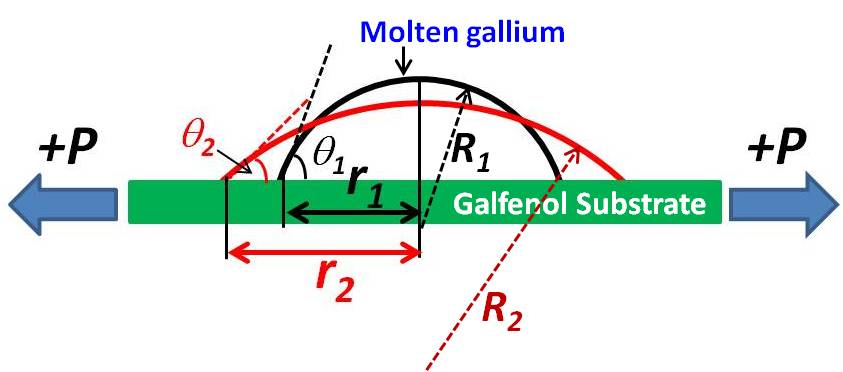
\includegraphics[width=\textwidth,trim={0 2cm 0 0}]{thermal-expand-drop}
	%	\caption{Thermal expansion of drop}
		\label{fig:thermal-expand-drop}
	\end{subfigure}
	\caption{Schematics indicating notation used and contact angles $\theta_{i}$, radii of drop-solid contact area $r_{i}$, and radii of curvature for a spherical drop $R_{i}$, for two temperatures as thermal expansion induced tension $P$ strains the substrate.}
	\label{fig:therm-exp-ga}
\end{figure}
The gallium drop contact angle technique uses classic contact angle measurement techniques and drop size analysis on a liquid metal, gallium, resting on a metal surface as the metal is heated. Figure \ref{fig:therm-exp-ga} illustrates the experiment. Gallium was chosen as the probe liquid for our high surface energy metals, \gamSV $\sim$2000 mJ/m$^2$, because it is a liquid above 29.8\degree C and it has an average surface tension of $\gamma_{Ga}\sim$715.3 mJ/m$^2$.\cite{Hardy1985} This means that liquid Ga will not completely wet a bare metal surface as water does. Water has a relatively low surface tension, $\gamma_{water}\sim$72.0 mJ/m$^2$, compared to a solid metal surface energy, hence when interacting with a bare metal surface the water contact angle will reduce to zero, and no solid surface energy can be calculated, which can be seen in Equation \ref{young_eqn}. The surface tension of Ga varies by 5 mJ/m$^2$ in the temperature range that this experiment will be carried out, $\sim$30-100\degree C, and will be accounted for in the final surface energy calculation. Ga surface tension can be linear plotted as $\gamma_{Ga} = 709 - 0.066(T-29.8)$, where $T$ is the temperature and 29.8 is the melting point of Ga.\cite{Hardy1985} A plot of Ga surface tension vs. temperature from Hardy \etal is shown in Figure \ref{fig:se-vs-temp-ga}. 

%%%%%%%%%%%%%%%%%%%
%This paragraph explains the choice of gallium as a probe liquid in a contact angle experiment for a metal surface instead of water. 
%It establishes Ga as a main contributor to the experiment. One that must be characterized well. 
%%%%%%%%%%%%%%%%%%%


\begin{figure}
	\centering
	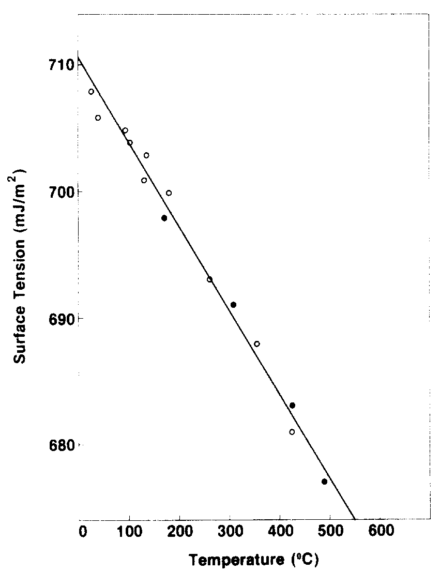
\includegraphics[width=0.5\linewidth,trim={0 0 0 1cm}]{se-vs-temp-ga}
	\caption{This figure plots the surface tension of pure Ga as temperature increases. This figure is from Hardy \etal \cite{Hardy1985}.}
	\label{fig:se-vs-temp-ga}
\end{figure}


Surface energy of FeGa will be calculated at temperatures ranging from 30-100\degree C in 10\degree C intervals. Changes in surface energy are introduced by thermal expansion of the substrate. By expanding the distance between atoms at the surface of the solid, the solid surface energy decreases. Intuitively, this makes sense because as the metallic bond distance increases, the less energy it would take to break those bonds. Electrons will begin to localize around the nuclei, as the attractive forces between atoms will decrease with the increased atomic separation. Ultimately, it will become easier for the metal to cleave and form two new surfaces, hence the surface energy decreases as temperature increases. 

Since a heated sample thermally expands, we can say that there is a tensile force on the edges of the stationary droplet of Ga. The triple point at every point of the droplet contact radius expands outward due to the thermal expansion of the probed surface. This tensile load can be called $ +P(T) $, seen in Figure \ref{fig:therm-exp-ga}, which effectively appears as a uniform radial force of the planar solid surface as temperature increases. By slowly heating the system by $\sim$1\degree C/min, the substrate expands uniformly while equilibrating at each temperature. Hence, terms due to variation in thermal energy and variation of the total Gibbs free energy are negligible. 

The surface energy of the substrate as a function of temperature, $\gamma_{SV}(T)$, can be related to $ +P(T) $ through the changes in the liquid Ga drop contact angle $\theta$, the radius $ r $ of the liquid gallium drop in contact with the metal surface, and the height $ h $ of the droplet hemisphere. A video system is used to precisely quantify dimension changes in substrate and liquid metal drop during thermal expansion.
%%%%%%%%%
%this paragraph introduces the model of finding solid surface energy from the gallium drop experiment. 
%
%As temperature is increased, a force is exerted on the triple line of the gallium sessile drop by the thermal expansion of the substrate.
%%%%%%%%%

The interfacial energy between the substrate solid and the liquid gallium drop, \gamSL, can be written as \gamSL$=P(T)/2\pi r$. The uniform tension introduced by thermal expansion of substrate can be expressed as:
\begin{equation}\label{uniform-tension}
	P(T) = E_{sub}\alpha_{sub}(T-T_{mp})
\end{equation}
where $T_{mp}$ is the melting temperature of gallium, $E$  is the substrate Young’s modulus, and $\alpha$ is the linear thermal expansion coefficient. A linear function can be used to write the gallium-air interfacial tension a function of temperature, \gamLV $= a-b(T-T_{mp})$, where \textit{a} and \textit{b} are positive constants found experimentally.\cite{Hardy1985,Alchagirov2005} Putting the terms for \gamSL and \gamSV into \hyperlink{youngeqn}{Young’s equation}\cite{Rudawska2009,Tadmor2004}:
\begin{equation*}%\label{youngs-eqn-ga1}
	\gamma_{SV} =  \frac{E_{sub}\alpha_{sub}(T-T_{mp})}{2\pi r} + \left[a-b(T-T_{mp})\right]\cos\theta
\end{equation*}
%%%%%%%%%%%%%%%%%%%%%
%Fully derives the gallium drop surface energy equation.
%This paragraph needs to be partially combined with the previous paragraph. 
%%%%%%%%%%%%%%%%%%%%%


A relationship between the variable radius $r(T)$ associated with the area of the circular region of solid-liquid contact $A_{SL}(T)$, the contact angle $\theta(T)$ and the volume $V$ of the spherical cap formed by the drop is derived next. To determine the radius $r(T)$, the geometric relationships based on the radius of curvature $R(T)$ of a sphere is mapped onto the hemispherical liquid cap. The drop is modeled as being part of a sphere whose radius is $R(T)$. It is assumed that he volume $V$ of the drop is the volume of the spherical cap, and remains constant. The radius $R(T)$ can then be expressed in terms of the volume and the angle:
\begin{equation*}\label{drop-geom}
	R(T) = V^{1/3} \left[\frac{\pi}{3} \left(2-3\cos\theta(T)+\cos^{3}\theta(T)\right)\right]^{-1/3}
\end{equation*}
Using the relation $r(T)=R(T)\sin\theta(T)$ (i.e. $\theta=$0\degree corresponds to complete wetting of the surface and at $\theta=90$\degree,  $r=R$) the following formula for surface energy as a function of temperature $T$ and contact angle $\theta(T)$ (shown as $\theta_{T}$) is:
\begin{equation}\label{youngs-eqn-ga}
	\gamma_{SV} =  \underbracket{\frac{E_{sub}\alpha_{sub}(T-T_{mp})}{2\pi}\left[\frac{\pi\left(2-3\cos\theta_{T}+\cos^{3}\theta_{T}\right)}{3V\sin^{3}\theta_{T}} \right]^{1/3}}_{\text{\gamSL(T)}} + \underbracket{\left[a-b(T-T_{mp})\right]}_{\text{\gamLV(T)}} \cos\theta_{T}
\end{equation}
This gives the surface energy \gamSV of specific grains as a function of temperature by measuring $T$ and $\theta$ at thermal equilibrium.



